\section{Parameter Efficiency with CNNs}

\subsection{CNN Implementation}

\begin{itemize}
    \item Final validation accuracy: \textbf{99.03\%}
    \item Number of parameters: \textbf{421,642}
    \item Training time: \textbf{4.8 minutes}
\end{itemize}

\begin{figure}[h]
    \centering
    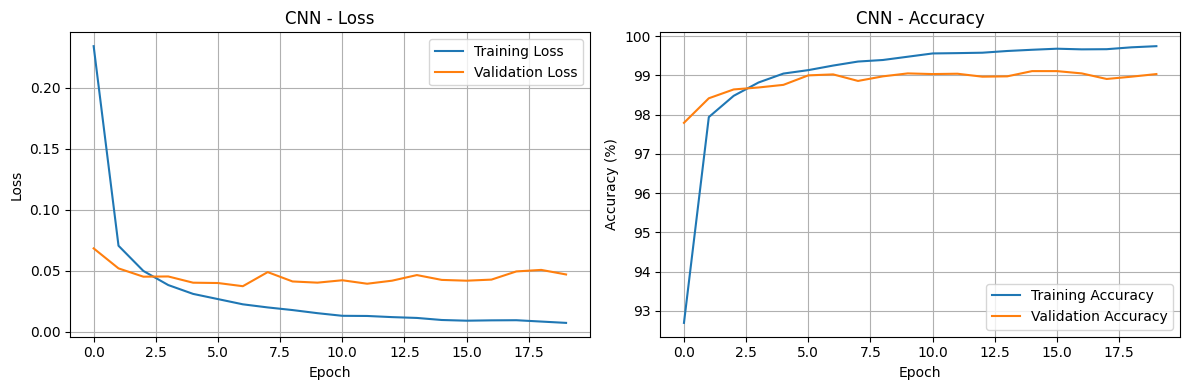
\includegraphics[width=0.7\linewidth]{section3/cnn.png}
    \caption{Training and validation curves for CNN model}
    \label{fig:cnn}
\end{figure}

\subsection{Question 3.1: Parameter Comparison}

\begin{table}[h]
\centering
\begin{tabular}{|l|c|c|c|}
\hline
\textbf{Model} & \textbf{Parameters} & \textbf{Val Acc} & \textbf{Train-Val Gap} \\ \hline
MLP (Dropout) & 535,818 & 98.31\% & 1.08\% \\ \hline
CNN & 421,642 & 99.03\% & 0.77\% \\ \hline
\end{tabular}
\caption{CNN vs MLP comparison}
\label{tab:cnn-comparison}
\end{table}

The CNN has 21.3\% fewer parameters (114,176 reduction) than the MLP.

\subsection{Question 3.2: Why do CNNs perform better?}

Even with fewer parameters, the CNN gets better validation accuracy (99.03\% vs 98.31\%) and shows less overfitting. This makes sense because CNNs are designed specifically for images:

First, CNNs keep the 2D structure of the image intact. When we use an MLP, we flatten the 28×28 image into a single list of 784 pixels, which loses information about which pixels are next to each other. CNNs use convolutional layers that process the image in its original 2D form, so they can detect patterns like edges and shapes more naturally. 

Second, CNNs have something called weight sharing where the same filter slides across the entire image. This means a CNN can recognize a digit whether it's in the top-left corner or bottom-right corner. Plus, this sharing makes CNNs way more efficient, a 3×3 filter needs only 288 parameters while a fully-connected layer would need 25,088 for the same job.

The results speak for themselves: the CNN has 21.3\% fewer parameters, 0.72\% better accuracy, and less overfitting (0.77\% gap vs 1.08\%).
